\documentclass[11pt,a4paper]{article}

\usepackage[margin=0.7in]{geometry}

\usepackage[utf8]{inputenc}
\usepackage{graphicx}
\usepackage{microtype}
\usepackage{float}
\usepackage{rotating}
\usepackage{xcolor}
\usepackage{sectsty}
\usepackage{url}
\usepackage{hyperref}

\usepackage{minted}

\hypersetup{
    colorlinks=true,
    linkcolor=blue,
    filecolor=magenta,      
    urlcolor=blue,
}

\urlstyle{same}
\definecolor{darkgray}{rgb}{0.66, 0.66, 0.66}
\definecolor{blue(ryb)}{rgb}{0.01, 0.28, 1.0}
\definecolor{dimgray}{rgb}{0.41, 0.41, 0.41}
\sectionfont{\color{cyan}} 
% \subsectionfont{\color{blue}}



\renewcommand{\texttt}[1]{%
  \begingroup
  \ttfamily
  \begingroup\lccode`~=`/\lowercase{\endgroup\def~}{/\discretionary{}{}{}}%
  \begingroup\lccode`~=`[\lowercase{\endgroup\def~}{[\discretionary{}{}{}}%
  \begingroup\lccode`~=`.\lowercase{\endgroup\def~}{.\discretionary{}{}{}}%
  \catcode`/=\active\catcode`[=\active\catcode`.=\active
  \scantokens{#1\noexpand}%
  \endgroup
}

\title{SOEN6461 - Software Design Methodology\\
Design Project\\
Group 9 - Deliverable 3\\
\bigskip
\large{\centerline{\textbf{Professor Yann-Gaël Guéhéneuc}}}
}

\begin{document}

\date{}
\maketitle



% \bigskip
% \bigskip

\begin{table}[H]
\centering
\begin{tabular}{|l|l|}
\hline
\textbf{Student ID} & \textbf{Unique email}               \\ \hline
40124288   & plablisenter@outlook.com   \\ \hline
40089008   & user.40089008@gmail.com    \\ \hline
40091878   & SOEN6461cheraghi@gmail.com \\ \hline
40130791   & komal3194p@gmail.com       \\ \hline
\end{tabular}
\end{table}

% \vspace{25em}

% \centerline{Department of Computer Science and Software Engineering}

% \centerline{Gina Cody School of Engineering and Computer Science}

% \centerline{Concordia University}

% \clearpage

\section{Analysis and Design Requirements}

On the one hand, the PADL meta-model allows describing models of (object-oriented) programs.

On the other hand, “PlantUML is a component that allows to quickly write : […] class diagrams” (See \url{https://plantuml.com/}).

Analyze, design, and implement a Visitor that generates a textual description of any PADL model. The description should include \texttt{padl.kernel.IFirstClassEntity} (and possibly all \texttt{padl.kernel.IEntity}) as nodes. The arcs between nodes should describes the different relations between entities (see \texttt{padl.kernel.IRelationship} and its sub-interfaces). The description should conform to the syntax and semantics of \url{https://plantuml.com/classdiagram} so that PlantUML can be called on this description. Demonstrate your implementation by providing textual description of some PADL model as well as the corresponding PlantUML-generated class diagrams.

\section{Implementation}

\subsection{Create PADL model}

The PADL library contains an interface called \texttt{padl.kernel.ICodeLevelModel}. The implementation class of this interface capable of holding the whole PADL meta-model of a set of related classes.

To populate the meta-models, we use the \texttt{create(final ICodeLevelModelCreator aCodeLevelModelCreator)} method, with combination with the \texttt{padl.creator.classfile.CompleteClassFileCreator} class. The source code for creating meta-model is already provided by professor Yann-Gaël Guéhéneuc. We put it inside a singleton class \texttt{plantumlgenerator.utils.MetaModelCreator}. Since the provided source code is just a code snippet, many libraries are required to make it run.

\subsection{Resolve dependencies}

Here is the list of dependencies that are missing/required
\begin{itemize}
    \item package \texttt{padl.kernel} for various interfaces and classes of meta-model.
    \item package \texttt{padl.analysis} for \texttt{UnsupportedSourceModelException}
    \item package \texttt{padl.creator.classfile} for class \texttt{CompleteClassFileCreator}.
    \item package \texttt{padl.statement.creator.classfiles} for using the class \texttt{ConditionalModelAnnotator} and \texttt{LOCModelAnnotator}
    \item package \texttt{padl.util} for using the class \texttt{ModelStatistics}
\end{itemize}

Each of these package have an corresponding project in \url{https://github.com/ptidejteam/v5.2} repository. Each project also have some dependencies on other libraries as well. To allow separation of each project, we convert each corresponding project into a Maven project and use Maven package command (\texttt{mvn package}) to create jar files.

Finally, we all all the jar files to \texttt{libs} folder of the main project, then add the dependency in Maven's \texttt{pom.xml} file with \texttt{<scope>} attribute set to \texttt{system}.

The dependency in \texttt{pom.xml} file should look like this and repeated with appropriate for every required libraries:

\begin{minted}[mathescape,
               linenos,
               numbersep=5pt,
               gobble=2,
               frame=lines,
               framesep=2mm]{xml}
    <dependency>
      <groupId>padl-lib</groupId>
      <artifactId>padl-lib</artifactId>
      <version>5.2</version>
      <scope>system</scope>
      <systemPath>${basedir}/libs/padl.jar</systemPath>
    </dependency>
\end{minted}

For the two package \texttt{padl.creator.classfile} and \texttt{padl.statement.creator.classfiles}, we must use the source code (not jar files) to prevent exception of type \texttt{java.lang.NoClassDefFoundError} when trying to load a folder of java compiled \texttt{.class} files. This make the project must be develop using Eclipse IDE. In the future, we will make the project IDE independent using Gradle or Maven.

\subsection{Implement the \texttt{padl.visitor.IGenerator} interface}

We decided to implement the \texttt{padl.visitor.IGenerator} interface for the job, because this interface provide the method \texttt{getCode()}. The \texttt{padl.visitor.IWalker} provide the method \texttt{Object getResult()}, which is not really fit for the task we are trying to do.

We created an abstract class \texttt{plantumlgenerator.visitor.PlantUmlVisitor}. The concrete class \texttt{plantumlgenerator.visitor.PlantUmlGenerator} will extend this abstract class and implements \texttt{padl.visitor.IGenerator}

\begin{figure}[H]
\centering
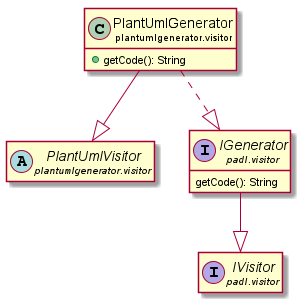
\includegraphics[scale=0.75]{diagrams/implement.png}\color{dimgray}
\caption{The class diagrams of implementation of \texttt{padl.visitor.IGenerator}}
\end{figure}

\subsubsection{Interested \texttt{open()} and \texttt{close()} methods}

Not all \texttt{open()} and \texttt{close()} methods in \texttt{padl.visitor.IGenerator} were used in the implementation. We only modify these couples of \texttt{open()} and \texttt{close()} methods (all the interfaces use as parameter in open() and close() methods are in \texttt{padl.kernel} package):

\begin{itemize}
    \item open and close for \texttt{IAbstractModel}: \texttt{IAbstractModel} is the root in the hierarchy of PADL meta-model. So we put the generation of beginning of plantuml code in the open() method, and put ending code in the close() method.
    \item open and close for \texttt{IPackageDefault} and \texttt{IPackage}: these two interfaces have the same implementation of plantuml code generation. The interface \texttt{IPackageDefault} is for "out of source code" packages (i.e. dependencies package). The \texttt{IPackage} is for normal packages that get compiled.
    \item open and close for \texttt{IGhost}: \texttt{IGhost} is for classes that have source code in the dependencies libraries (i.e. \texttt{java.io.Serializable})
    \item open and close for \texttt{IClass}: \texttt{IClass} is for classes that have source code compiled into .class file.
    \item open and close for \texttt{IInterface}: \texttt{IInterface} is for interfaces that have source code compiled into .class file.
\end{itemize}

\subsubsection{Plantuml code structure and creation}

A typical plantuml source code is follow:

\begin{minted}[frame=lines,framesep=2mm]{text}
@startuml diagram_name

' Packages, classes and interfaces declaration

package packageName {
    class className {
    }
    abstract abstractClassName {
    }
    interface interfaceName{
    }
}

' Classes and interface relationship

className ..|> interfaceName
className --|> abstractClassName

@enduml

\end{minted}

To generate plantuml source code using this template, we use two \texttt{java.lang.StringBuffer}. One for the packages, classes and interface declaration. The other one is for classes and interfaces relationship. The relationship string buffer is only append text in \texttt{open()} methods. Finally, at the \texttt{close(IAbstractModel arg0)} method, we append the relationship string buffer to the declaration string buffer. This kind of implementation allow us to have plexible algorithm to generate code, decouple the responsibilities of each \texttt{StringBuffer} object.

In the end, we return the declaration string buffer with \texttt{toString()} method in \texttt{padl.visitor.IGenerator.getCode()} method.

\clearpage

\subsubsection{All classes are inherited from \texttt{java.lang.Object}}

An interesting problem occurred on generated plantuml code. All java class are extended from \texttt{java.lang.Object} class. This make the diagram over complicated. Therefore, we need to handle the case of class is \texttt{java.lang.Object} in relationship string buffer.

The \texttt{padl.kernel.IClass} have \texttt{getName()} method (inherited from \texttt{padl.kernel.IFirstClassEntity}). Comparing the class name with "Object" allow us to distinguish between a normal class with \texttt{java.lang.Object} class.

\section{How to run the project and coding convention}

\subsection{Coding convention}

The coding convention can be found here:

\url{https://github.com/huntertran/soen6461-plantuml-generator/wiki/Coding-Conventions}

Since that is a private repository, an exact copy of the document can be found in this public repository:

\url{https://github.com/huntertran/soen6441-riskgame/wiki/Coding-Conventions}

\subsection{How to run the project}

The project must be run from Eclipse IDE.

\begin{itemize}
    \item Step 1: extract the zip file and import all 3 project into new Eclipse workspace by select the root folder
    
\begin{figure}[H]
    \centering
    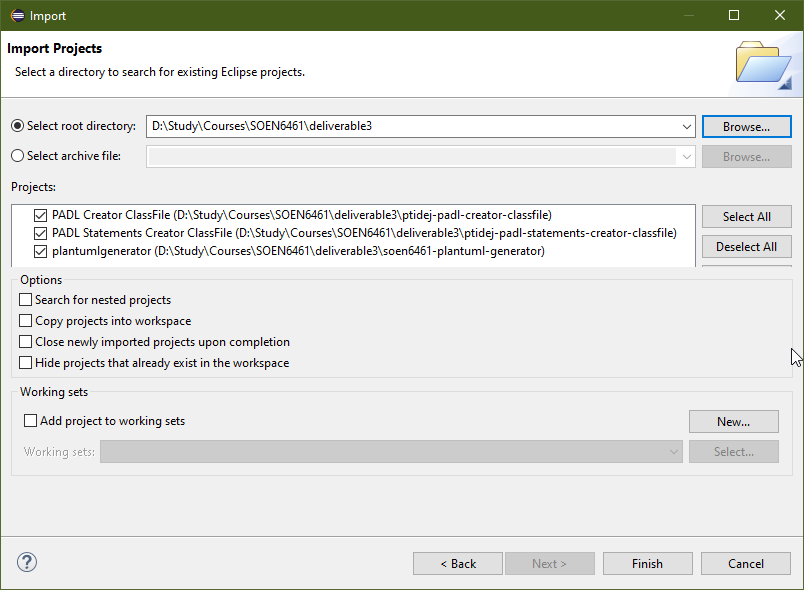
\includegraphics[scale=0.5]{images/open_project.png}\color{dimgray}
    \caption{Import all 3 folder into new eclipse workspace}
\end{figure}
    
    \item Step 2: Select \texttt{plantumlgenerator}. Choose Run / Run As / Java Application
    
\begin{figure}[H]
    \centering
    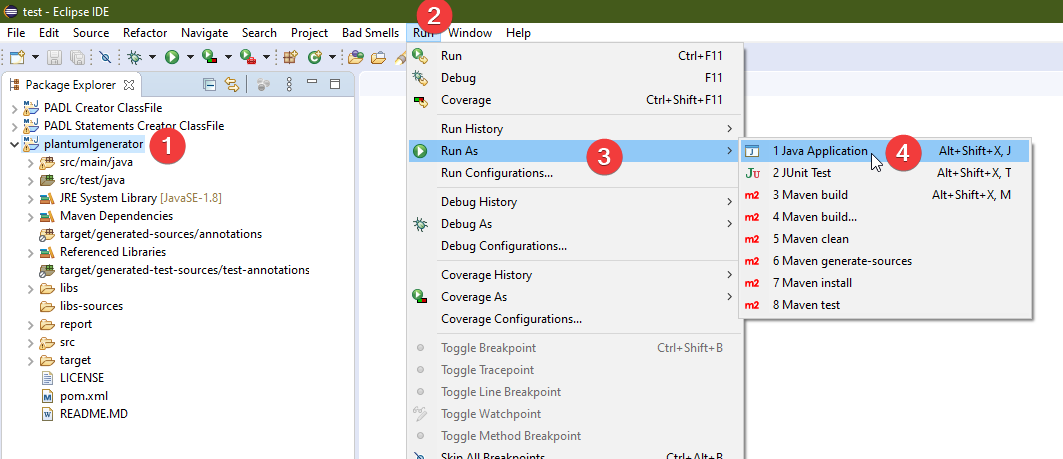
\includegraphics[scale=0.5]{images/run_as.png}\color{dimgray}
    \caption{\texttt{plantumlgenerator} run as Java Application}
\end{figure}

\begin{figure}[H]
    \centering
    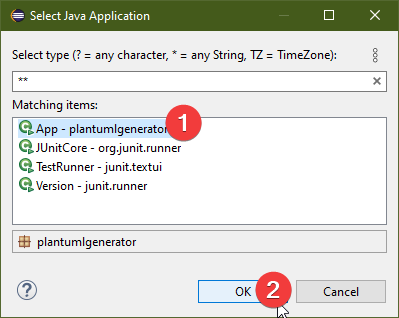
\includegraphics[scale=0.5]{images/main_app.png}\color{dimgray}
    \caption{Choose the target App}
\end{figure}

    \item Step 3: copy and paste the path to the compiled .class files.\\
    An example to test is "./src/test/java/plantumlgenerator/padl/event/"\\
    Enter "n" to show the result in a new window (for copy)
    
\begin{figure}[H]
    \centering
    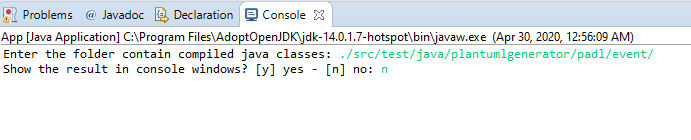
\includegraphics[scale=0.5]{images/console.png}\color{dimgray}
    \caption{enter the target folder contains compiled .class files}
\end{figure}

\begin{figure}[H]
    \centering
    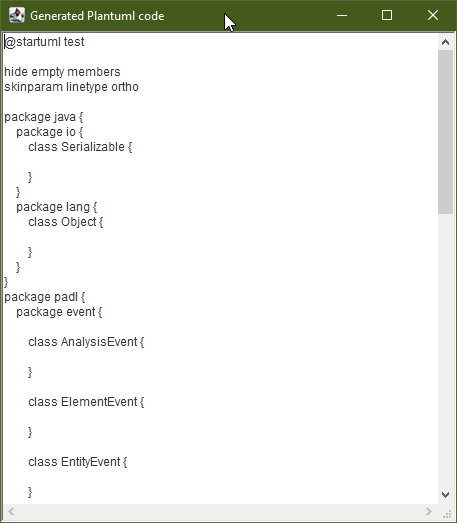
\includegraphics[scale=0.5]{images/result.png}\color{dimgray}
    \caption{Show the result in new window}
\end{figure}

    \item Step 4: [Optional] View the diagram online at \url{http://www.plantuml.com/plantuml/uml/}
    
\end{itemize}

The result diagram for \texttt{./src/test/java/plantumlgenerator/padl/event/} folder can be viewed \href{http://www.plantuml.com/plantuml/uml/ZL9BRi8m4DtFANm1E0DTe0gfLHTTT8Sq90CCiSUHFKHAA-vUegQMcBfIl60nxyFJUzbanQJNu9rILe0pj-Gez3gwGE50AKFkM7fC69nd8HrxSZ7fEGBqs7Hu8dV10TqNkFlxFN6S3lDhFERitYanUlx4WwSxMD0RbDyYzoYdFmPlXmirMfFUIfGUMs-Yq40ogOpRaw0VC-UjXM-MkVKKI7G1KPHrNC2R6Cyab51Z-eVAefIEs93RrHmhjDVOad_Xh9Fp4hhoiQwfXTwr97S1DwWSfHR9y6M87LbUTUs1C_yKOIm-q7UKwei3F2wuNk_dfW3AOXOe2vcxMMI2vZ-lOG-VCW3KgbojzcOH0B0TsXYbCtFVaBJNuBy1}{here}.

\begin{figure}[H]
    \centering
    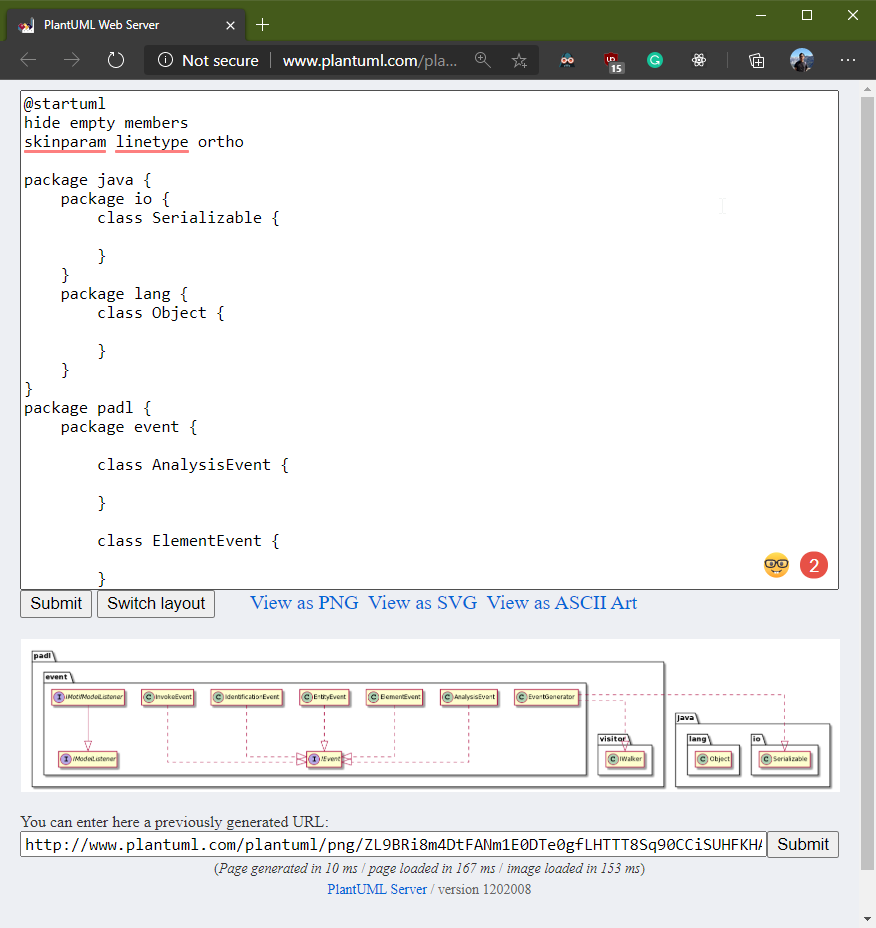
\includegraphics[scale=0.5]{images/diagram.png}\color{dimgray}
    \caption{The online diagram generator}
\end{figure}

\end{document}
